We want to develop a terrain generation algorithm and corresponding viewer. 

Our main inspiration for this project is the article by Patel\cite{redblob}.
The author presents an algorithm for generating terrain maps for games based on certain game design decisions.
Figure~\ref{fig:map-2d} gives an example of a terrain map that was generated by the demonstration implementation of the algorithm.

\begin{figure}[H]
	\centering
	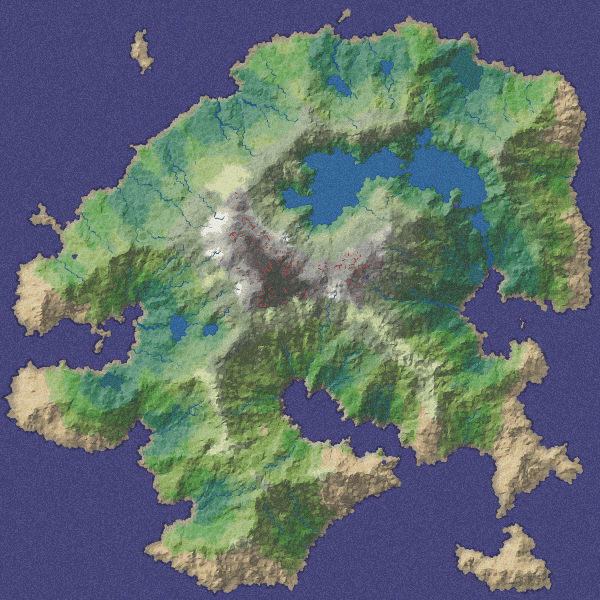
\includegraphics[width=\linewidth]{map-2d}
	\caption{An example terrain}
	\label{fig:map-2d}
\end{figure}

While we do not intend to follow the same general rules for terrain generation, the author gives a clear description of the algorithm which we should be able to use to develop an algorithm for our specific use case.
Most importantly, the goal in the paper is to generate a mountainous island that gets higher the further one goes inland.
While this is not a bad approximation of reality, we feel it is too strong, and that it results in terrains that are not easily explored 'on foot'.

The author makes some interesting suggestions for future work.
In Section~\ref{sec:func}, we will list what feature we want to add to the terrain generator.

Our only requirement for the terrain viewer is that it should be able to easily explore the generated terrain.
We will at least implement a mode for 'walking', but we may add more feature if this enables easier exploration.

The terrain generation algorithm is the focus of our project.

The author of \cite{redblob} does not give any way to explore the terrain.
The demonstration implementation does however have a few different terrain viewers, among which is a 3D viewer, shown in Figure~\ref{fig:map-3d}.
We do not want to implement these simple viewers, though they might be useful for debugging.

\begin{figure}[H]
	\centering
	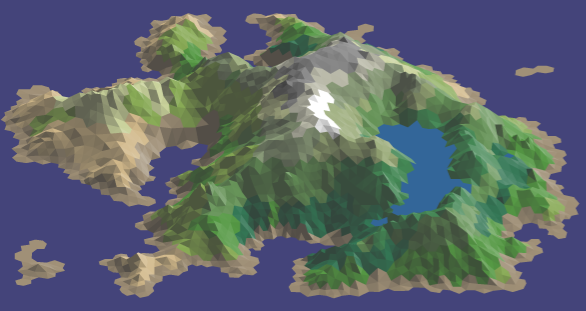
\includegraphics[width=\linewidth]{map-3d}
	\caption{A 3D render of the map depicted in Figure~\ref{fig:map-2d}}
	\label{fig:map-3d}
\end{figure}

